\documentclass[12pt,fleqn]{article}\usepackage{../../common}
\begin{document}
Materyel Mekaniği - 4

Yapıların stres, kaykılma fiziğini kullanarak Euler-Bernoulli kirişlerinden
bahsedildi, ve bir diferansiyel denklem elde edildi. Bu denklem kesin (exact)
olarak çözülebilir fakat bazı durumlarda çözümü zor olabilir. Kesin metotlar
yerine yaklaşık metotlara bakmak faydalı olacaktır.

Rayleigh-Ritz metotu diferansiyel denklemleri yaklaşıksal olarak çözmenin bir
yöntemidir. Metot bunu sistemin potansiyel enerjisi $\Pi$'yi minimize ederek
yapar [1, Ders 3]. Potansiyel enerji sistemin toplam iç gerilme enerjisi eksi
sistem üzerinden yapılan iş olarak hesaplanabilir,

$$
\Pi = \int_\Omega \overline{U} \ud x - W
$$

Bu noktada aklımıza pek çok soru gelebilir - niye potansiyel enerji minimize
ediyoruz, iş gerilme enerjisi ve yapılan iş nasıl hesaplanır, potansiyel enerji
nasıl minimize edilir gibi..

Potansiyel Enerji ve Denge

İlk önce denge bağlamında potansiyel enerjinin ne demek olduğunu işleyelim.

Potansiyel enerji $\Pi$ sistemin stabilitesi ile alakalıdır. Mesela alttaki
resim stabilite konusunu işleyen her ders kitabında vardır, bir kapta duran topu
aldım, yukarı doğru çıkatıp (bordo renk) aşağı bıraktım, top kabın dibine gidip
orada kalacaktır (kırmızı renk). 

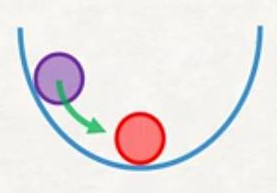
\includegraphics[width=10em]{phy_020_strs_04_01.jpg}

Yani top ilk denge konumuna dönecektir, ve o durumda potansiyel enerjisi minimum
olmuştur deriz ve bu denge stabil bir dengedir.


\includegraphics[width=10em]{phy_020_strs_04_02.jpg}

İkinci durumda topu orta noktada sola taşırız, top orada kalır, bu yeni
bir denge noktasıdır, $\Pi$ değişmemiştir, burada nötr bir denge vardır.

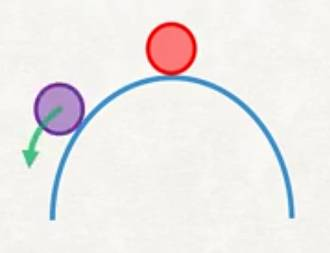
\includegraphics[width=10em]{phy_020_strs_04_03.jpg}

Üçüncü durumda ters kavisli bir yüzey var, top üst orta noktadan başlıyor
diyelim (orada durması zor olsa da), topu yine alıp sola taşıyorum, top aşağı
düşecektir. Üstteki durum potansiyel enerjisinin maksimum olduğu bir durumdur,
sistem stabil değildir. Rayleigh-Ritz yönteminin amacı (potansiyel enerjinin
minimum olduğu) stabil denge durumunu hedefleyerek bir yaklaşık çözüme
ulaşmaktır.

Bunu nasıl yaparız? Daha önce belirttiğimiz potansiyel enerjinin iki bileşeni
var, ilki sistemin toplam iç gerilim (deformasyon) enerjisi. Gerilim enerji
{\em yoğunluğu} $\overline{U}$ genel olarak bir materyelin stres-gerilim eğrisinin
altındaki alan olarak hesaplanabilir.

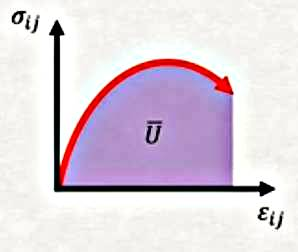
\includegraphics[width=10em]{phy_020_strs_04_04.jpg}

Mesela üstteki gibi stres $\sigma_{ij}$ ve gerilim $\epsilon_{ij}$ arasındaki
bir eğriyi düşünelim, bu eğrinin altında kalan alan, yani entegral hesabı 
gerilim enerji yoğunluğunu verir.

$$
\overline{U} = \int_{0}^{\epsilon_{ij}} \sigma_{ij} \ud \epsilon_{ij}
$$

Kolaylaştırıcı bir faktör, bizim bu derste kullanacağımız maddeler lineer
elastik, yani stres-gerilim eğrisi alttaki gibi,

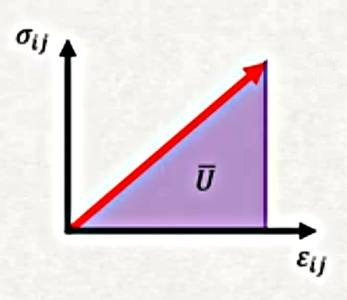
\includegraphics[width=10em]{phy_020_strs_04_05.jpg}

Bu durumda ``eğri'' yani çizgi altındaki alan basit bir üçgen hesabı,

$$
\overline{U} = \frac{1}{2} \sigma_{ij} \epsilon_{ij}
$$

Fakat bu sadece tek bir boyutu halletti, mesela üstteki örnek $e_1$ yönündeki
bir esnemeyi temsil ediyor olabilirdi, fakat 3 boyutlu ortamda elimizde daha
fazla bileşen olduğunu biliyoruz, $\sigma_{11}$ haricinde $\sigma_{22}$ var,
$\sigma_{33}$ var, $\sigma_{12}$, $\sigma_{23}$, vs.. Tüm stres/gerilim
eşleri için [2, Ders 16],

$$
\overline{U} = \frac{1}{2} \sum_{i,j=1}^{3} \sigma_{ij} \epsilon_{ij}
$$

Toplamı açarsak,

$$
= \frac{1}{2} (\sigma_{11}\epsilon_{11} + \sigma_{22}\epsilon_{22}  +
\sigma_{33}\epsilon_{33} + \sigma_{12}\epsilon_{12} + \sigma_{23}\epsilon_{23} +
\sigma_{13}\epsilon_{13} + \sigma_{33}\epsilon_{33} + \sigma_{23}\epsilon_{23} +
\sigma_{32}\epsilon_{32} )
$$

Son ifadeyi daha basitleştirmek mümkün, $\sigma$ ve $\epsilon$'un simetrik
olduğunu unutmayalım,

$$
\overline{U} = \frac{1}{2} (\sigma_{11}\epsilon_{11} + \sigma_{22}\epsilon_{22}  +
\sigma_{33}\epsilon_{33} + 2 \sigma_{12}\epsilon_{12} +
2 \sigma_{13}\epsilon_{13} + 2 \sigma_{23}\epsilon_{23} )
$$

Üsttekileri mühendislik gerilimi $\gamma_{ij} = 2 \epsilon_{ij}$ ile temsil
etmek mümkün,

$$
\overline{U} = \frac{1}{2} (\sigma_{11}\epsilon_{11} + \sigma_{22}\epsilon_{22}  +
\sigma_{33}\epsilon_{33} + \sigma_{12}\gamma_{12} +
\sigma_{13}\gamma_{13} + \sigma_{23}\gamma_{23} )
$$
 
[atlandı]

Eksenel Yükleme (Axial Loading)

Euler-Bernoulli kiriş formülasyonu sadece bükülmenin sebep olduğu deformasyonu
hesaba kattı, bunu yaparken nötr eksen üzerindeki eksenel deformasyonu yok saydı
[3, 8.4]. Euler-Bernoulli modelini eksenel yatay deformasyonu hesaba katacak
şekilde genişletmek mümkündür, fakat, belki de bu iyi haber, ufak deformasyon
önkabulü sayesinde eksenel yük ve bükülme deformasyonları birbirinden
bağlantısız (uncoupled) hale gelir, eksenel yük sadece eksenel deformasyonu,
yatay yük sadece yatay deformasyonu etkiler.

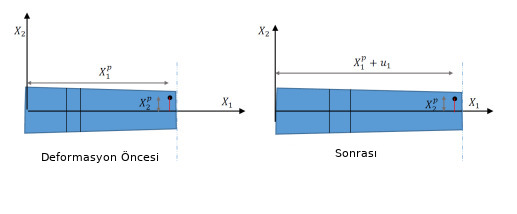
\includegraphics[width=25em]{phy_020_strs_04_06.jpg}

Diğer faraziyeler Euler-Bernoulli modeline benzer, düzlem bölümler düzlem kalır,
Poisson oranı etkileri yok sayılır, ve yatay yer değişimi $u_1$ pürüzsüz bir
fonksiyondur. Farklı bir resmi [2, Ders 15] eklersek,

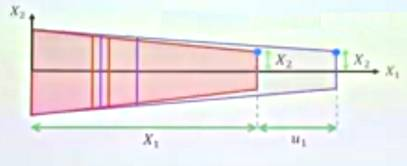
\includegraphics[width=20em]{phy_020_strs_04_08.jpg}

Bu faraziyelerle modeli oluşturalım; üstteki resme bakarsak $u_1 = u_1(X_1)$, ve
pozisyon vektör fonksiyonu olarak,

$$
x = \left[\begin{array}{c}
X_1 + u_1 \\ X_2 \\ X_3
\end{array}\right]
$$

Bu durumda yer değişim fonksiyonu

$$
u = x - X = \left[\begin{array}{c}
u_1 \\ 0 \\ 0
\end{array}\right]
$$

Hatırlarsak yaklaşık olarak gerilim tensörü

$$
\epsilon = \frac{1}{2} (\nabla u + \nabla u^T )
$$

Gradyanlar ile hesabı yaparsak sadece $\epsilon_{11}$'in sıfır olmadığını
görüyoruz,

$$
\epsilon = \left[\begin{array}{ccc}
\frac{\ud u_1}{\ud X_1} & 0 & 0 \\
0 & 0 & 0 \\
0 & 0 & 0 
\end{array}\right]
\mlabel{1}
$$

Bize gerekli diferansiyel denklemi kuvvet dengelerine bakarak ortaya
çıkartabiliriz. Şimdi kirişin $\ud X_1$ genişliğindeki ufak bir parçasına
odaklanalım,

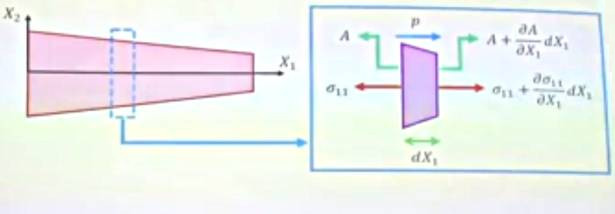
\includegraphics[width=20em]{phy_020_strs_04_07.jpg}

Bu parçanın sol ve sağındaki kuvvetlere bakarsak üstteki resim ortaya çıkar.

Oklar sola ya da sağa doğru gösterildi çünkü mesela $\sigma_{11}$ ve
$\sigma_{11} + \frac{\partial \sigma_{11}}{\partial X_1} \ud X_1$'in
birbirini dengeleyeceklerini / birbirlerine karşı ortaya çıktıklarını
biliyoruz, sağa doğru olan $p$ zaten dışarıdan uygulanan eksenel kuvvet.
$\frac{\partial \sigma_{11}}{\partial X_1}$ kullanımı $\sigma_{11}$'in
$X_1$'e oranla değişim hesabı için kullanıldı, bu oranı $X_1$'deki
olan değişimle çarpınca (örnekte $\ud X_1$) tabii ki ufak parçanın sağındaki
$\sigma_{11}$ eki ortaya çıkıyor, bunu $\sigma_{11}$'e topluyoruz.

Parçanın sol ve sağındaki alan büyüklüğü benzer şekilde, solda $A$ varsa
$A$'nin $X_1$'e oranlı değişimi çarpı $X_1$ değişimi bize parçanın sağındaki
alan büyüklük ekini veriyor. 

$X_1$ ekseni bazındaki denge denklemi o zaman alttaki gibi olur, stres hesabı
kuvvet bölü birim alan olduğu için kuvveti elde etmek için stres çarpı alan
gerekeceğini hatırlayalım, ayrıca $p$ kuvveti birim $X_1$ bazlı alınıyor,
o zaman $p \ud X_1$ kullanmak gerekir,

$$ \sum F_{X_1} = - \sigma_{11} A +
\left( \sigma_{11} + \frac{\partial \sigma_{11}}{\partial X_1} \ud X_1  \right)
\left( A + \frac{\partial A}{\partial X_1} \ud X_1  \right) + p \ud X_1 = 0
$$

Formülü açarsak

$$
-\sigma_{11} A  + \sigma_{11} A  +
\sigma_{11} \frac{\partial A}{\partial X_1} \ud X_1 +
A \frac{\partial \sigma_{11}}{\partial X_1} \ud X_1 +
\frac{\partial A}{\partial X_1} \frac{\partial \sigma_{11}}{\partial X_1} \ud X_1^2 +
p \ud X_1 = 0
$$

$\sigma_{11} A$ terimleri iptal olur,

$$
\sigma_{11} \frac{\partial A}{\partial X_1} \ud X_1 +
A \frac{\partial \sigma_{11}}{\partial X_1} \ud X_1 +
\frac{\partial A}{\partial X_1} \frac{\partial \sigma_{11}}{\partial X_1} \ud X_1^2 +
p \ud X_1 = 0
$$

$\ud X_1$ dışarı çekilir, ve sağda sıfır olduğu için iptal edilebilir,

$$
\sigma_{11} \frac{\partial A}{\partial X_1}  +
A \frac{\partial \sigma_{11}}{\partial X_1}  +
\frac{\partial A}{\partial X_1} \frac{\partial \sigma_{11}}{\partial X_1} \ud X_1 +
p  = 0
$$

Hala basitleştirme mümkün, dikkat edersek $\ud X_1$ terimini kullandık ve
ona ``çok küçük bir parça'' dedik. Bu parçayı sonsuz küçültürsek, yani
limiti alırsak, ki $\ud X \to 0$, o zaman üstteki formülde üçüncü terim
yokolur,

$$
\sigma_{11} \frac{\partial A}{\partial X_1}  +
A \frac{\partial \sigma_{11}}{\partial X_1}  
p  = 0
$$

Daha kısa bir formüle ulaştık. Fakat bize lazım olan yer değişimi, üstteki
formülde bu yok. Oraya ulaşmaya çalışalım. Dikkat edersek üstteki formülde
ilk iki terim sanki Calculus'ta çarpım kuralının açılmış haline benziyor,
o zaman o kuralı ters yönde işletirsek, yani gruplama amaçlı geriye gidersek,

$$
\frac{\partial }{\partial X_1} (\sigma_{11} A ) + p = 0
$$

Şimdi $\sigma_{11} = E \epsilon_{11}$ formülünü hatırlayalım, bu nereden geldi?
Elimizde bir tekeksenel yük var, o zaman en baz stres-gerilme ilişkisi geçerli
olur, yerine koyarsak,

$$
\frac{\partial }{\partial X_1} (E \epsilon_{11} A ) + p = 0
$$

Peki $\epsilon_{11}$ nedir? Bu büyüklüğü (1)'de gördük, $\epsilon$'un tek sıfır
olmayan öğesi $\epsilon_{11}$ ve orada $\frac{\ud u_1}{\ud X_1}$ değeri
var. Bunu üstteki formüle koyalım,

$$
\frac{\partial }{\partial X_1} \left( E A \frac{\ud u_1}{\ud X_1} \right) + p = 0
$$

Böylece içinde yer değişimi içeren bir formül elde etmiş oldum, $u_1$ yer
değişimidir.

Bu denklemi artık çözüm için kullanabiliriz. Tasarımcı olarak biz Young'in
Genliği $E$'yi biliriz, kirişin herhangi bir noktasındaki satıhsal alan $A$'yi
biliriz, kirişe uygulanan yük $p$'yi biliriz, tüm bunları kullanarak yer değişim
$u_1$'i üstteki formülle bulabiliriz. Tek bilinmeyen $u_1$ çünkü.

Şimdi bu noktada bazı püf noktalar ortaya çıkıyor; çünkü eğer $E,A$ büyüklükleri
$X_1$'in fonksiyonu iseler çözüm daha karmaşık hale gelebilir çünkü üstteki
formülde dış türev $X_1$'e göre. Fakat şimdiye kadar bu derste $X_1$'e bağlı bir
$E$ görmedik, yani Young'in Genliği kirişin her noktasında aynı, özetle sabit.
Sabit ise $E$ diferansiyelin dışına alınabilir. $A$ aynı şekilde. Eğer $A$
değişken ise o zaman Calculus çarpım kuralı uygularız.

O zaman iki senaryo şöyle olabilir, $E$ sabit ama $A$ değil,

$$
E \frac{\partial A}{\partial X_1} \frac{\partial u_1}{\partial X_1} +
EA \frac{\partial^2 u_1}{\partial X_1} + p = 0
$$

Hem $E$ hem $A$ sabit,

$$
E A \frac{\partial^2 u_1}{\partial X_1} + p = 0
$$










[devam edecek]

Kaynaklar

[1] Petitt, {\em Intro to the Finite Element Method}, University of Alberta,
    \url{https://www.youtube.com/watch?v=2iUnfPRk6Ro&list=PLLSzlda_AXa3yQEJAb5JcmsVDy9i9K_fi}

[2] Petitt, {\em Intro to the Continuum Mechanics}, University of Alberta,
    \url{https://www.youtube.com/playlist?list=PLLSzlda_AXa3N5jaDART7kimBlYz1dFnX}

[3] Adeeb, {\em Introduction to Solid Mechanics}
    \url{https://engcourses-uofa.ca/books/introduction-to-solid-mechanics/}
    
[5] Khennane, {\em Introduction to Finite Element Analysis Using MATLAB and Abaqus}

\end{document}


